\section{Examples}
\justify
The use of generalized state space models has multiple applications. In (\cite{song2007correlated}) several applications are presented.

\subsection{Generalized State Space Models for Longitudinal Binomial Data}
In some cases the data analysed in a time series are not observations extrapolated from a normal distribution but a binomial one, i.e. the presence or absence of a specific state.

In (\cite{kitagawa1987}) the Tokyo Rainfall Data is presented. The data is presenting the number of occurrences of rainfall over 1 mm in Tokyo as a proxy of a rainy versus non-rainy day. This is of course a type of non normal data and therefore might be modeled using a GSSM. In this case the use of a binomial distribution seems the best approach.
\par \vspace{5mm}
The equations governing the model are:
\begin{equation}
    \begin{gathered}
        Y_t|S_t \sim Bi(2, \pi_t) \text{ with } \pi_t = \sigma(S_t)\\
        S_t = S_{t-1} + \epsilon_t
    \end{gathered}
\end{equation}
The state process is therefore assumed to be a random walk. With these definitions the predicted time series using a Kalman predictor would be the following.

\begin{figure}
    \centering
    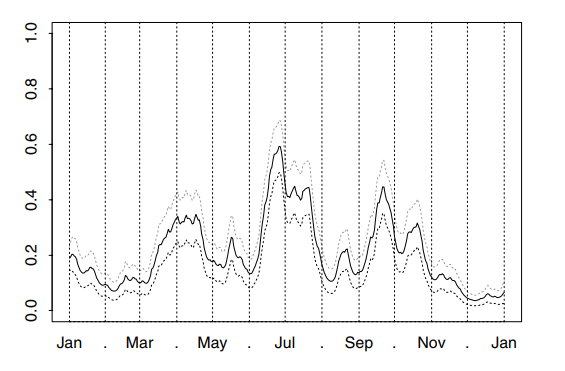
\includegraphics[width=8.5cm]{tokyo_rainfall.PNG}
    \caption{Monte Carlo predicted probability process based on the Kalman smoother proposed above}
    \label{fig:rain}
\end{figure}

The figure (\ref{fig:rain}) clearly indicates some kind of seasonal pattern over the year in Tokyo. The summer season seems to be the wettest for the city while winter is usually dry. The approach is fairly simple, but it relies on an additional step on top of what we already highlighted in the literature review (Equation \eqref{eq:distprob}). Once \textbf{P} is defined also the rest of the Kalman filter generalized quantities needs to be derived. This is:
\begin{equation}
    \textbf{P}_{t|t} = g_t(\textbf{S}_{t|t-1})\textbf{P}_{t|t-1}/\textbf{B}^t\textbf{P}_{t|t-1}\textbf{B}+\sigma^2
\end{equation}
As derived in (\cite{kitagawa1987} - Equation 2.3). From there, recursively applying the equations leads us to the discussed data.

\subsection{Generalized State Space Models for Longitudinal Count Data}

In some other cases the time series is related to count data. Again we cannot assume normality in such a case and we need GSSM to model the data.

In (\cite{Scot-1988}) we are presented with a count time series of poliomyelitis disease incidence over the US population between 1970 and 1983. We also observe the exposure to environments that might increase the risk of contracting the disease. In this case the measurement equation might take the form:
\begin{equation}
    Y_t|S_t \sim Po(a_t, S_t) \text{ with } a_t = e^{x_t^T\alpha}
\end{equation}
where 
\begin{equation}
\begin{gathered}
    x_t = (1, t, cos(2\pi t/12), sin(2\pi t/12), \\
    cos(2\pi t/6), sin(2\pi t/6))
    \end{gathered}
\end{equation}
In a similar fashion to what we discussed above, the authors of the paper derive a Kalman filter and smoother equations system to model the incidence of the data.

\begin{figure}
    \centering
    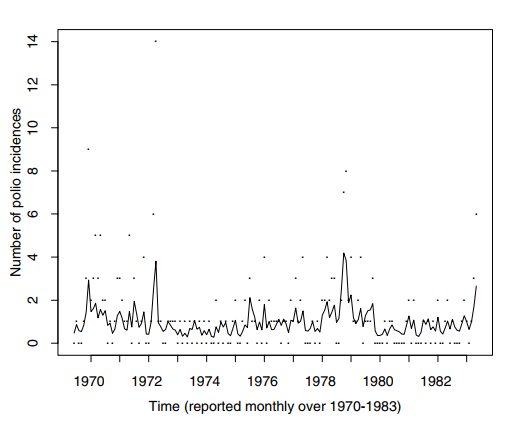
\includegraphics[width=8.5cm]{polio.PNG}
    \caption{Predicted probability process based on the Kalman smoother for the polio data. Dot shows observed counts and the solid line present the estimated process}
    \label{fig:polio}
\end{figure}

The  result is reassuring: the trend in the data is significantly different from zero and negative, showing a reduced impact of the disease on the population over time.